\chapter{Experimentos}
\label{cap:capitulo6}

En este capítulo se recogen las distintos experimentos que se han llevado a cabo durante el desarrollo del proyecto. Estas pruebas han sido fundamentales para verificar el correcto funcionamiento del sistema de reconocimiento de maduración de frutos y su comunicación con el brazo robótico, permitiendo así alcanzar los objetivos definidos en fases anteriores del trabajo.

\section{Detección con YOLOv3 y TensorFlow}
\label{exp_seleccion_algoritmo}

Dada la finalidad del proyecto, se requería que la detección de objetos se diera en tiempo real, por lo que se buscó información sobre YOLO, un sistema de código abierto que permitía esto a partir de una red neuronal convolucional para detectar objetos en imágenes y vídeo, y se iniciaron las pruebas pertinentes para la selección del algoritmo de detección y de las bibliotecas a utilizar.

\subsection{Pruebas con imágenes}
\label{sec:Pruebas_imgs_TF}

En primer lugar, se creó un entorno de Anaconda para poder probar la detección de objetos en imágenes utilizando Tensorflow mediante el repositorio \textit{deteccion\_objetos}\footnote{\url{https://github.com/puigalex/deteccion_objetos}} basados en la configuración \textit{faster rcnn resnet101 coco} de los modelos de detección de objetos de Tensorflow para poder llevar a cabo la comparación, y etiquetando imágenes, en este caso de tigres, mediante la herramienta labelImg\footnote{\url{https://github.com/HumanSignal/labelImg}}, se prepararon las carpetas y archivos de configuración correspondientes para poder llevar a cabo el entrenamiento del modelo siguiendo los pasos indicados en el repositorio utilizando una distribución de las imágenes utilizadas para el aprendizaje del modelo y su uso en la detecciónn aproximadamente del 70:30 (73\% datos de entrenamiento y 27\% datos de prueba)(Cuadro \ref{tab:Imagenes_Entrenamiento}), a partir de los cuales se entrenó ese 70\% con uno de los algoritmos y los respectivos parámetros escogidos y medimos su rendimiento usando el 30\% restante de los datos.

  \begin{table}[H]
  \centering
  \begin{tabularx}{\textwidth}{|X|X|X|}
    \hline
    \centering \textbf{Imágenes usadas en entrenamiento} & 
    \centering \textbf{Imágenes usadas en test} & 
    \centering \textbf{Número total de imágenes} \tabularnewline
    \hline
    \centering 594 & \centering 218 & \centering 812 \tabularnewline
    \hline
  \end{tabularx}
  \caption{Distribución de las imágenes utilizadas para el entrenamiento del modelo}
  \label{tab:Imagenes_Entrenamiento}
  \end{table}

Se entrenó este modelo hasta que se observó que la pérdida estaba por debajo de 1, considerando que esta pérdida no era alta, y que no existían demasiadas fluctuaciones,  deteniendo este entrenamiento a los 1400 pasos, a pesar de que este entrenamiento estuviera programado para llegar hasta los 20000, ya que se trataba de una prueba simplemente. Esto supuso que se tuviera que utilizar el último checkpoint disponible, en este caso el del paso 1337 (Figura \ref{fig:Deteccion_Prueba_TF}), para convertirlo en un modelo final y de esta manera poder generar predicciones, utilizando imágenes de diferentes tamaños.

  \begin{figure}[H]
    \begin{center}
      \subcapcentertrue
      \subfigure[Pasos finales del entrenamiento con TensorFlow]{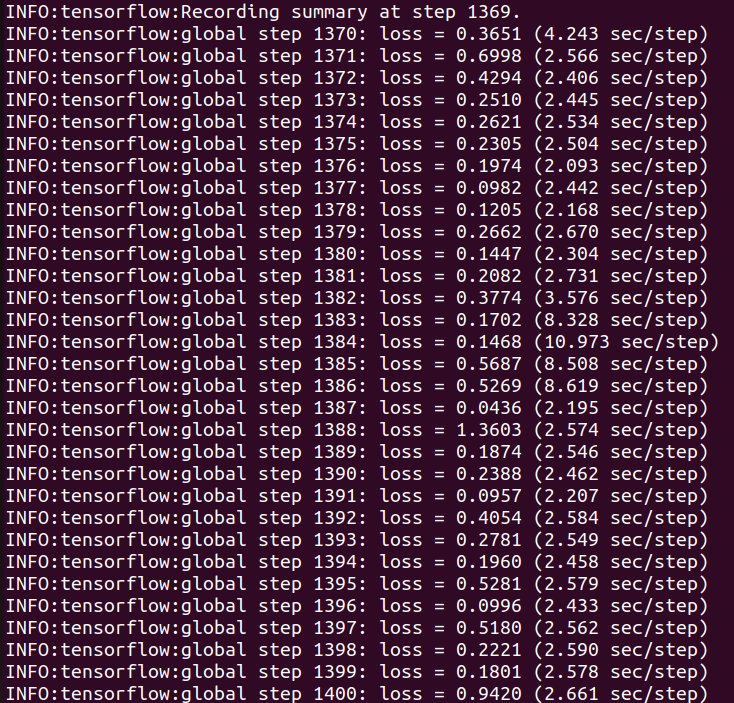
\includegraphics[height=50mm, width=70mm]{figs/Pasos finales del entrenamiento_TF.png}}
      \hspace{4mm}
      \subfigure[Checkpoints del entrenamiento con TensorFlow]{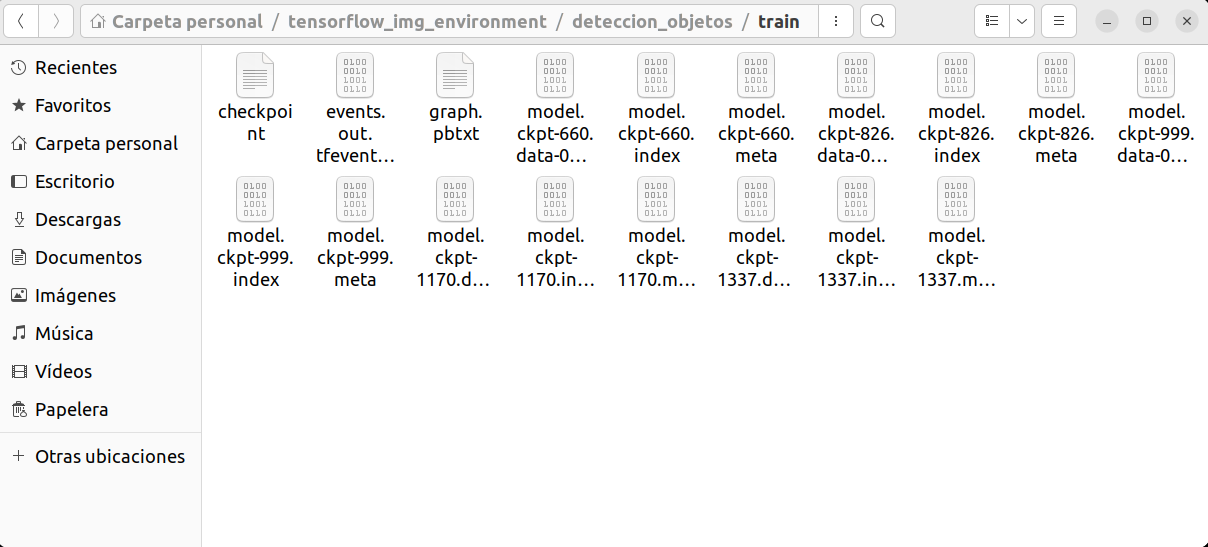
\includegraphics[height=50mm, width=70mm]{figs/checkpoints_TF.png}}
    \end{center}
    \caption{Entrenamiento del algoritmo con TensorFlow}
    \label{fig:Deteccion_Prueba_TF}
  \end{figure}
  
Una vez convertido el checkpoint en un modelo final, se procedió a realizar las primeras pruebas de detección en imágenes de este modelo, comprobando su capacidad para detectar correctamente los tigres para este caso, y evaluar visualmente los resultados obtenidos en algunos ejemplos mostrados en la Figura \ref{fig:deteccion_tensorflow_tigres}, de estas primeras detecciones realizadas tras el entrenamiento.

  \begin{figure}[H]
  \centering
  % Fila 1
  \begin{minipage}{0.46\textwidth}
    \centering
    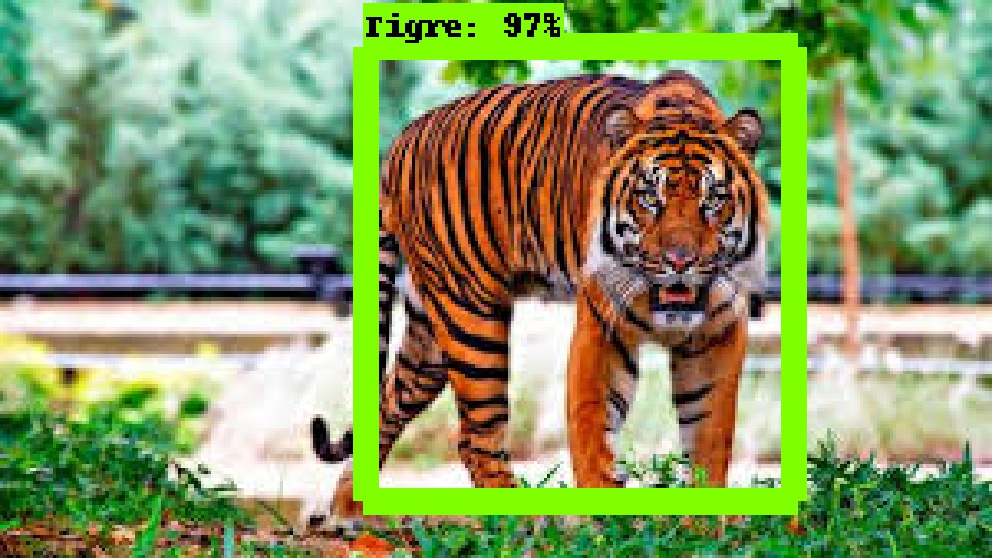
\includegraphics[width=\linewidth]{figs/tigre_1.jpeg}
  \end{minipage}
  \hspace{2mm}
  \begin{minipage}{0.46\textwidth}
    \centering
    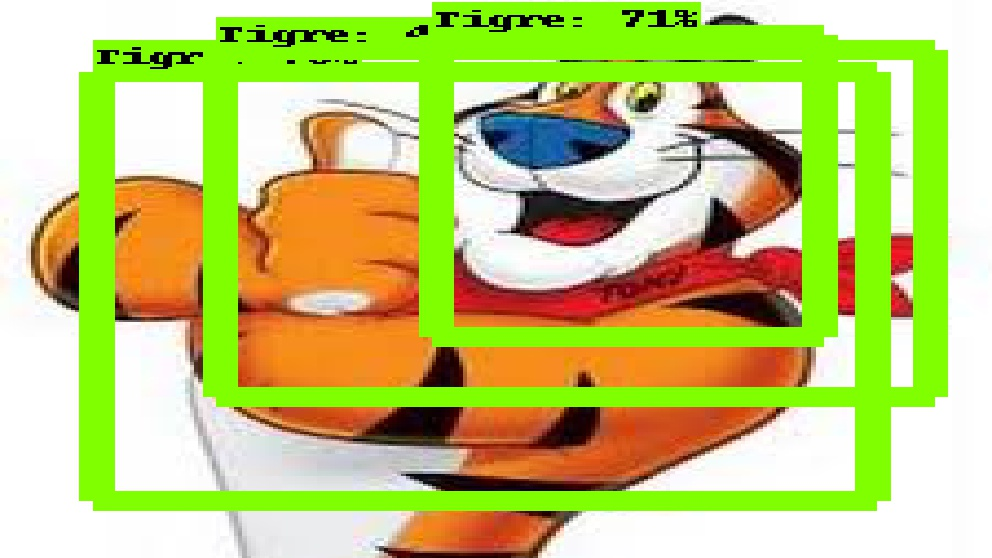
\includegraphics[width=\linewidth]{figs/tigre_2.jpeg}
  \end{minipage}
  \\[4mm] % Espacio vertical entre las dos filas
  % Fila 2
  \begin{minipage}{0.46\textwidth}
    \centering
    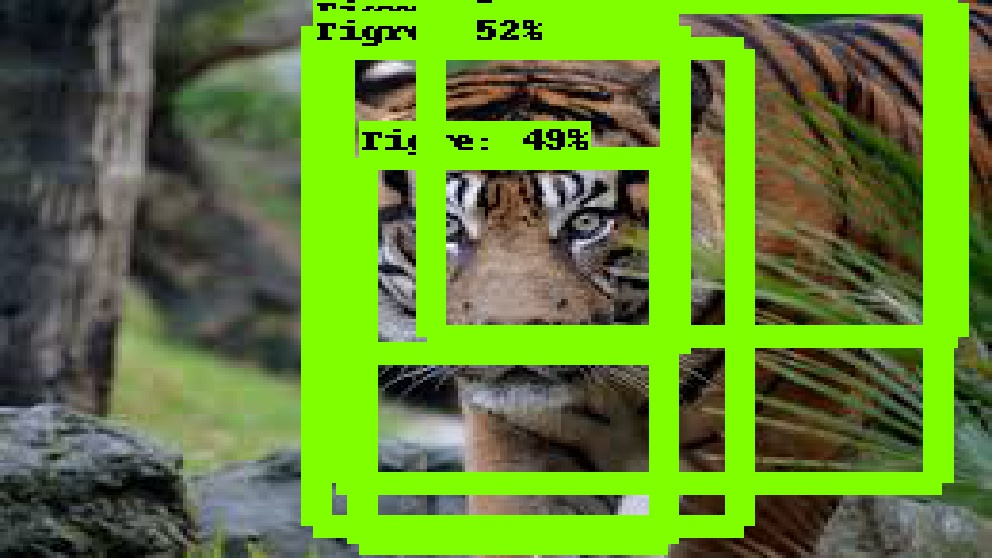
\includegraphics[width=\linewidth]{figs/tigre_4.jpeg}
  \end{minipage}
  \hspace{2mm}
  \begin{minipage}{0.46\textwidth}
    \centering
    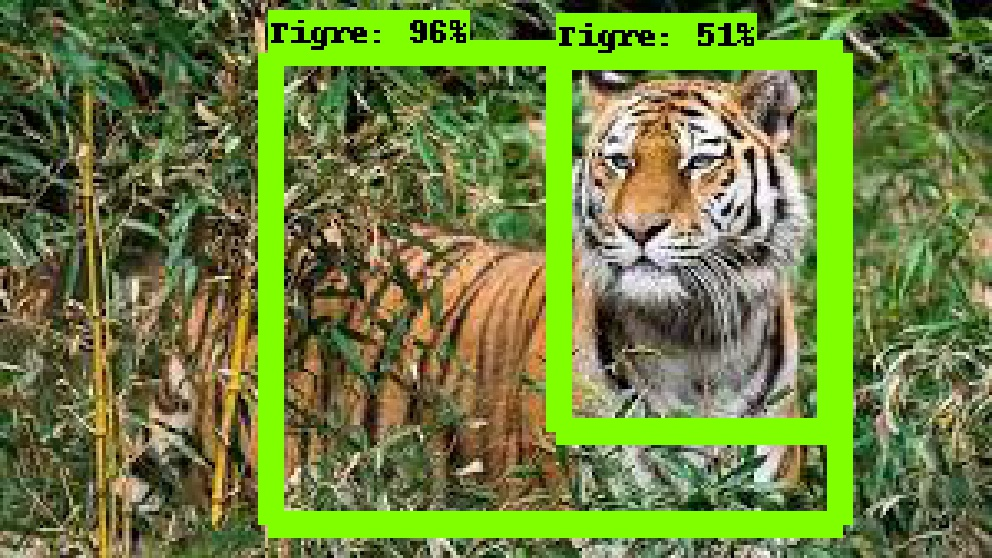
\includegraphics[width=\linewidth]{figs/tigre_5.jpeg}
  \end{minipage}
  \caption{Resultado de la detección en imágenes con TensorFlow}
  \label{fig:deteccion_tensorflow_tigres}
  \end{figure}
 
Dados los resultados obtenidos en las imágenes utilizadas para esta primera prueba, se decidió llevar a cabo un nuevo proceso de entrenamiento a partir del último checkpoint disponible con el objetivo principal de comprobar si, aumentando el número de pasos de entrenamiento, se lograba una mejora significativa tanto en la disminución del valor de pérdida como en el incremento del porcentaje de confianza en las detecciones realizadas. Así, se retomó el entrenamiento desde el checkpoint del paso 1337, extendiéndose en esta segunda ocasión hasta el paso 2945, momento en el cual se optó por detener manualmente el proceso al observarse una estabilización progresiva en los valores de pérdida, y siendo este último checkpoint generado fue el correspondiente al paso 2877, obteniéndose en este punto un valor de pérdida de tan solo 0.222, notablemente inferior al registrado en el primer intento. A continuación, se procedió a ejecutar nuevamente el programa sobre las mismas imágenes de prueba de tigres empleadas en la primera serie de tests, lo que permitió realizar una comparación directa entre ambos modelos, y observar que en esta segunda ejecución existía una clara mejora en la calidad de las detecciones, tanto en términos de mayor porcentaje de confianza como en la precisión de los cuadros delimitadores sobre los objetos detectados (ver Figura \ref{fig:deteccion_tensorflow_tigres_v2}).

  \begin{figure}[H]
  \centering
  % Fila 1
  \begin{minipage}{0.46\textwidth}
    \centering
    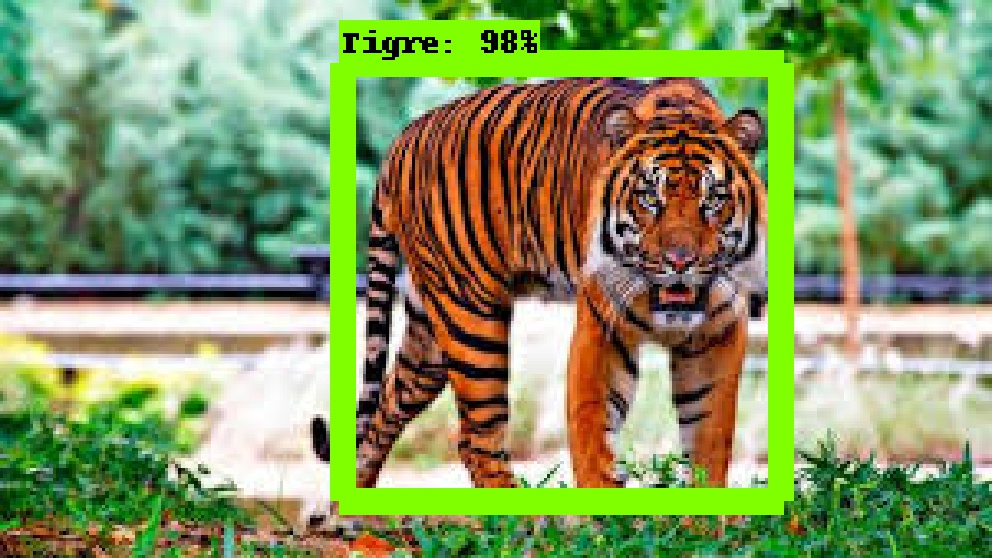
\includegraphics[width=\linewidth]{figs/tigre_1_v2.jpeg}
  \end{minipage}
  \hspace{2mm}
  \begin{minipage}{0.46\textwidth}
    \centering
    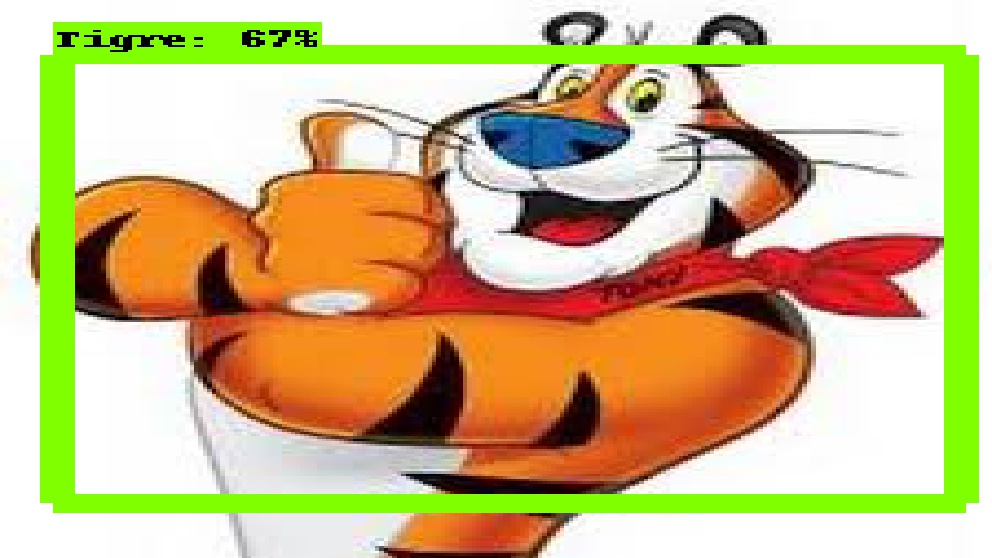
\includegraphics[width=\linewidth]{figs/tigre_2_v2.jpeg}
  \end{minipage}
  \\[4mm] % Espacio vertical entre las dos filas
  % Fila 2
  \begin{minipage}{0.46\textwidth}
    \centering
    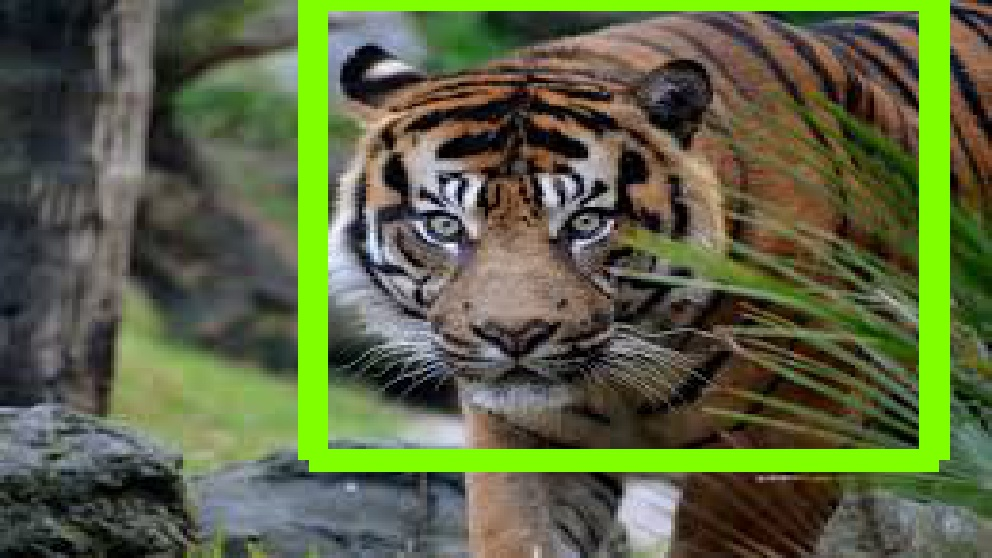
\includegraphics[width=\linewidth]{figs/tigre_4_v2.jpeg}
  \end{minipage}
  \hspace{2mm}
  \begin{minipage}{0.46\textwidth}
    \centering
    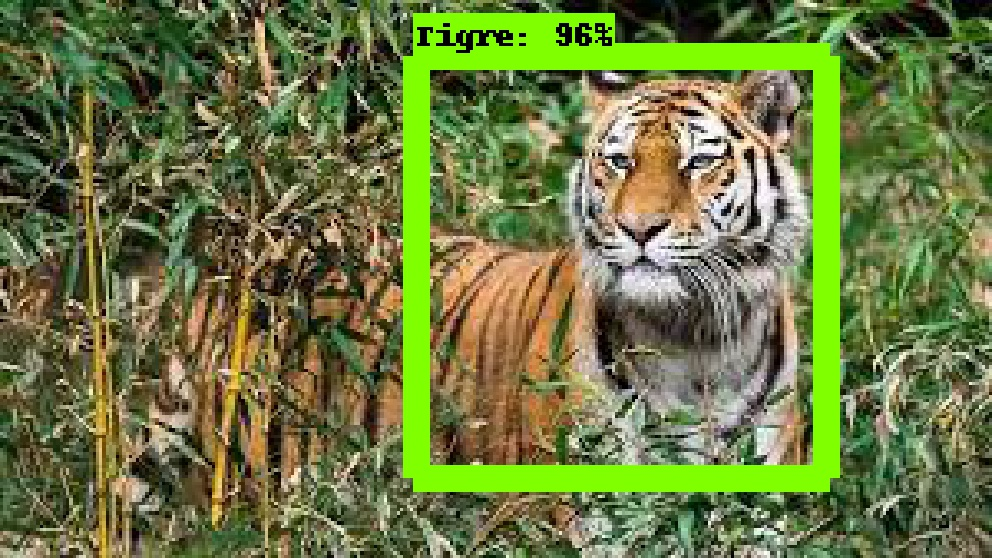
\includegraphics[width=\linewidth]{figs/tigre_5_v2.jpeg}
  \end{minipage}
  \caption{Resultado del reentrenamiento de la detección en imágenes con TensorFlow}
  \label{fig:deteccion_tensorflow_tigres_v2}
  \end{figure}


Después de llevar a cabo estas poruebas con el ejemplo de los tigres, se comprobó si el modelo funcionaría también con el objeto final, en este caso, con fresas, por lo que, a través de la página Kaggle, se obtuvo un dataset de 262 frutas\footnote{\url{https://www.kaggle.com/datasets/aelchimminut/fruits262}} de las cuales únicamente se utilizó el archivo de las fresas, que contenía 1002 imágenes para llevar a cabo estas pruebas.\\

Una vez descargado el archivo, se comenzó a etiquetar una a una las imágenes mediante la herramienta labelImg para obtener los archivos xml, tal y como se había hecho con el ejemplo anterior de los tigres, y antes de terminar de etiquetar el dataset entero, se probó este modelo utlizando las primeras 405 imágenes etiquetadas siguiendo una distribución de estas del 80:20 para su entrenamiento y usando el checkpoint guardado en el paso 3490 para congelar el modelo, y así poder utilizar varias imágenes aún por etiquetar para probarlo, obteniendo un resultado satisfactorio en cuanto a la detección y su confianza, tal y como se puede observar en la Figura \ref{fig:Deteccion_Fresas_Imagenes_TF}.

  \begin{figure}[H]
  \centering
  % Fila 1
  \begin{minipage}{0.45\textwidth}
    \centering
    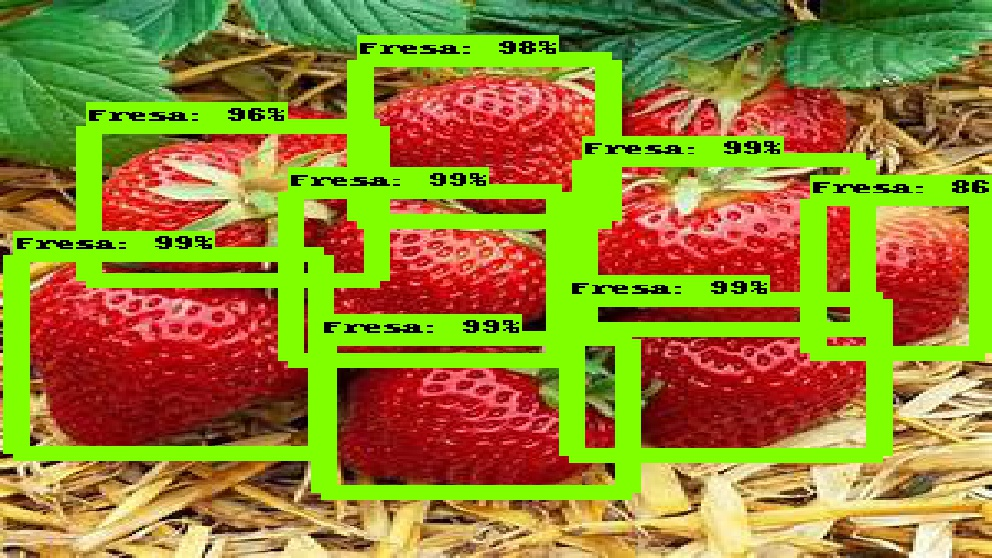
\includegraphics[width=\linewidth]{figs/999.jpeg}
  \end{minipage}
  \hspace{2mm}
  \begin{minipage}{0.45\textwidth}
    \centering
    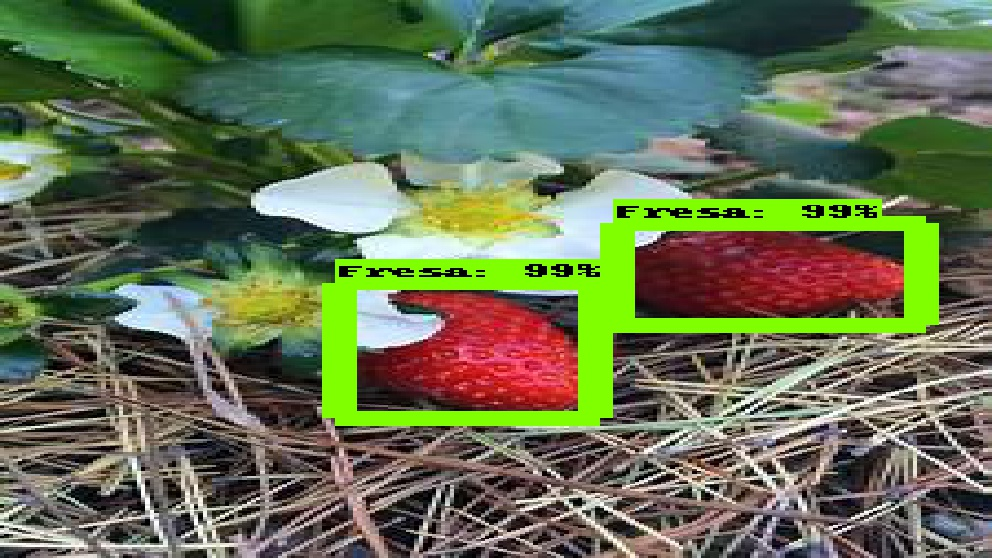
\includegraphics[width=\linewidth]{figs/947.jpeg}
  \end{minipage}
  \\[4mm] % Espacio vertical entre las dos filas
  % Fila 2
  \begin{minipage}{0.45\textwidth}
    \centering
    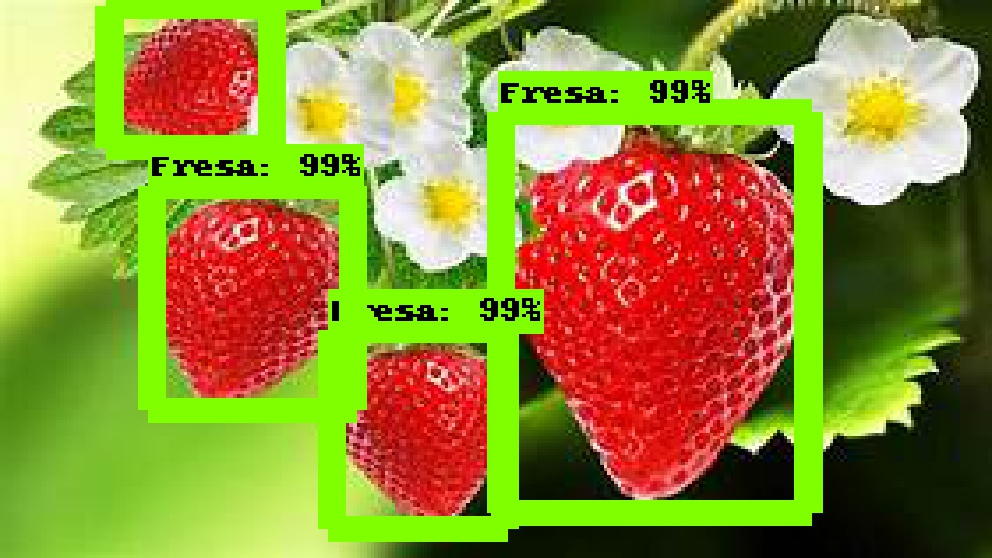
\includegraphics[width=\linewidth]{figs/868.jpeg}
  \end{minipage}
  \hspace{2mm}
  \begin{minipage}{0.45\textwidth}
    \centering
    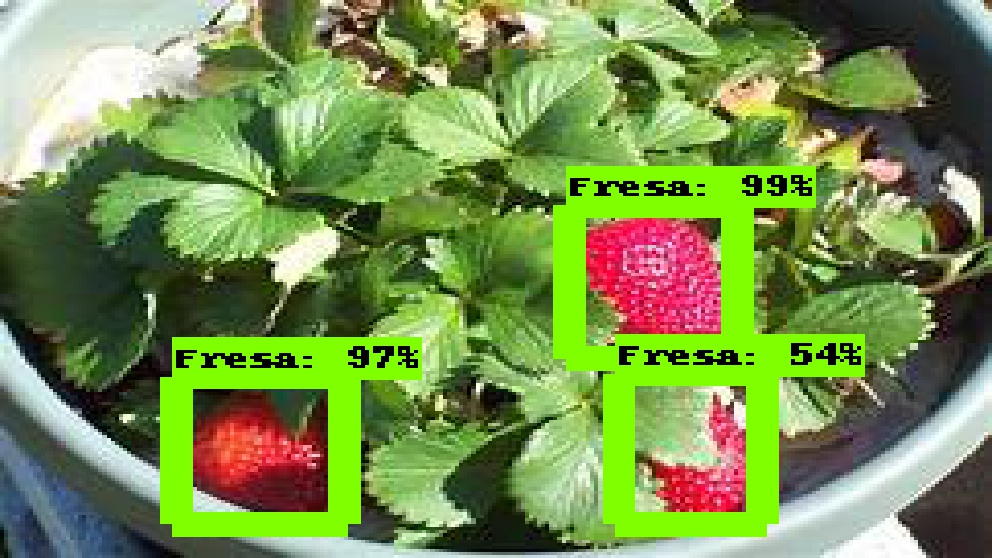
\includegraphics[width=\linewidth]{figs/1000.jpeg}
  \end{minipage}
  \caption{Pruebas de deteccion de fresas en imágenes con TensorFlow}
  \label{fig:Deteccion_Fresas_Imagenes_TF}
  \end{figure}

Tras haber conseguido la detección de fresas en imágenes estáticas utilizando TensorFlow, el siguiente paso dentro del desarrollo del sistema consistió en extender las pruebas a la detección en vídeo en tiempo real, por lo que, de forma análoga a como se había realizado previamente con la librería PyTorch, se procedió a evaluar distintos modelos de detección de objetos pertenecientes al zoo de TensorFlow (TensorFlow 2 Detection Model Zoo), los cuales, al estar ya preentrenados sobre conjuntos de datos de referencia, permitieron llevar a cabo una comparación de estos diferentes modelos o sistemas bajo las mismas condiciones iniciales sin necesidad de realizar un nuevo entrenamiento desde cero. 

\subsection{Pruebas con vídeo en tiempo real}
\label{sec:Pruebas_video_TF}

Para la realización de estas pruebas, se utilizó tanto la cámara web integrada del ordenador portátil como una imagen previamente seleccionada, para que, de esta manera pudieran observarse las diferencias entre los modelos tanto en la detección en vídeo como en la detección en imágenes, y poder valorar qué modelo de los tres distintos probados ofrecería mejores prestaciones en términos de precisión, velocidad de procesamiento y robustez frente a las condiciones reales de trabajo (ver Figuras  \ref{fig:modelo_ssd_mobilenet}, \ref{fig:modelo_efficientdet_d4} y \ref{fig:modelo_faster_rcnn_resnet50}). 

	\begin{figure}[H]
    		\begin{center}
      		\subcapcentertrue
      		\subfigure[Resultado del modelo en imagen]{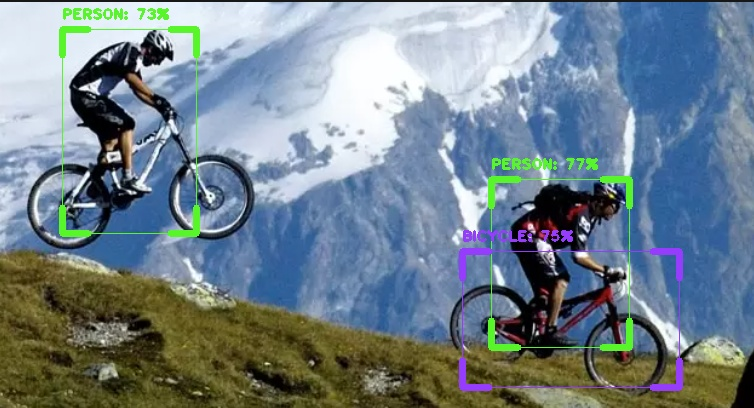
\includegraphics[height=50mm, width=70mm]{figs/ssd_mobilenet_v2_320x320_coco17_tpu-8.jpeg}}
      		\hspace{2mm}
      		\subfigure[Resultado del modelo en vídeo]{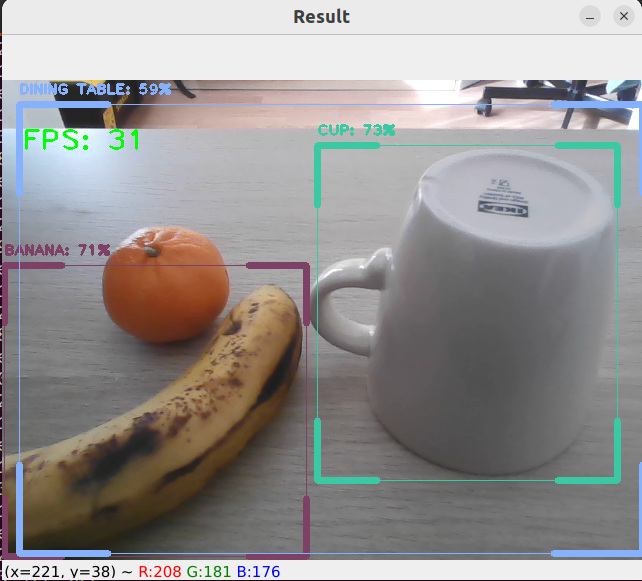
\includegraphics[height=50mm, width=70mm]{figs/webcam ssd_mobilenet_v2_320x320_coco17_tpu-8.png}}
    	\end{center}
    	\caption{Modelo ssd\_mobilenet\_v2\_320x320\_coco17\_tpu-8}
    	\label{fig:modelo_ssd_mobilenet}
  	\end{figure}
  	

  	\begin{figure}[H]
    		\begin{center}
      		\subcapcentertrue
      		\subfigure[Resultado del modelo en imagen]{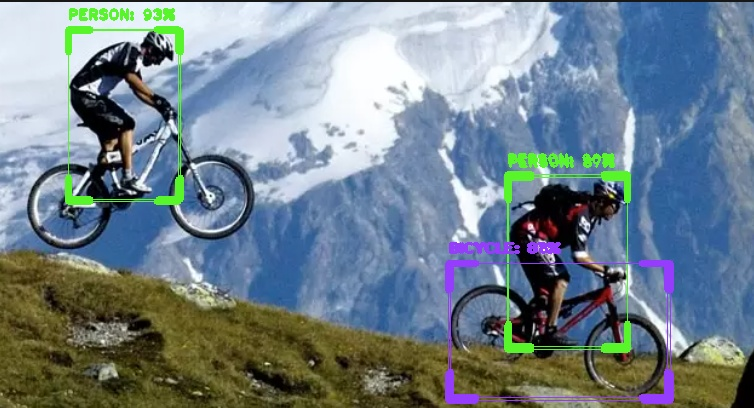
\includegraphics[height=50mm, width=70mm]{figs/efficientdet_d4_coco17_tpu-32.jpeg}}
      		\hspace{2mm}
      		\subfigure[Resultado del modelo en vídeo]{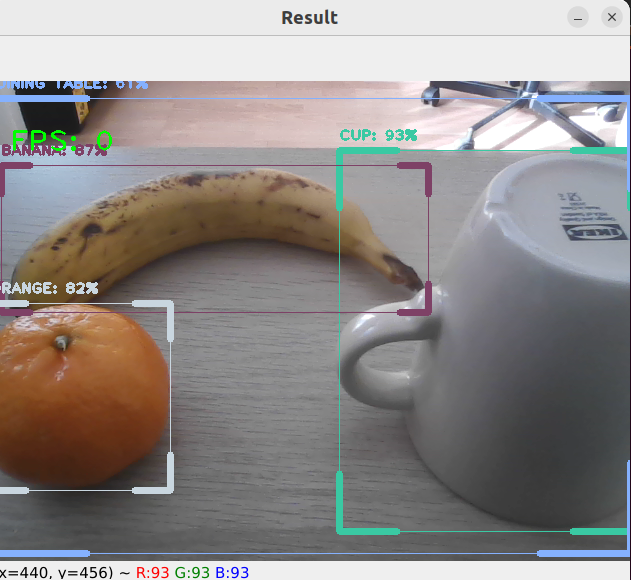
\includegraphics[height=50mm, width=70mm]{figs/webcam efficientdet_d4_coco17_tpu-32.png}}
    	\end{center}
    	\caption{Modelo efficientdet\_d4\_coco17\_tpu-32}
    	\label{fig:modelo_efficientdet_d4}
  	\end{figure}

  	\begin{figure}[H]
    		\begin{center}
      		\subcapcentertrue
      		\subfigure[Resultado del modelo en imagen]{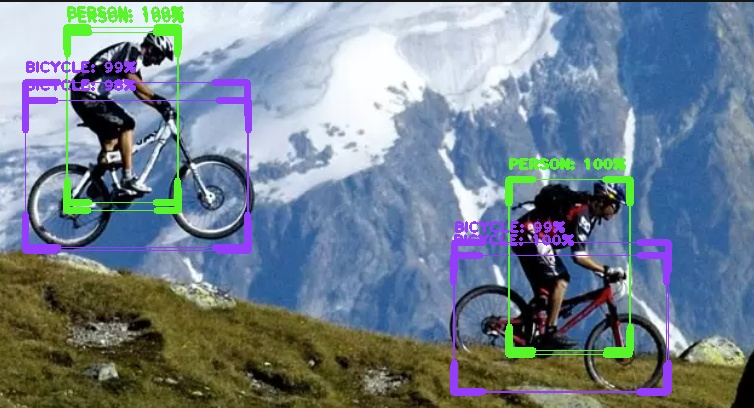
\includegraphics[height=50mm, width=70mm]{figs/faster_rcnn_resnet50_v1_640x640_coco17_tpu-8.jpeg}}
      		\hspace{2mm}
      		\subfigure[Resultado del modelo en vídeo]{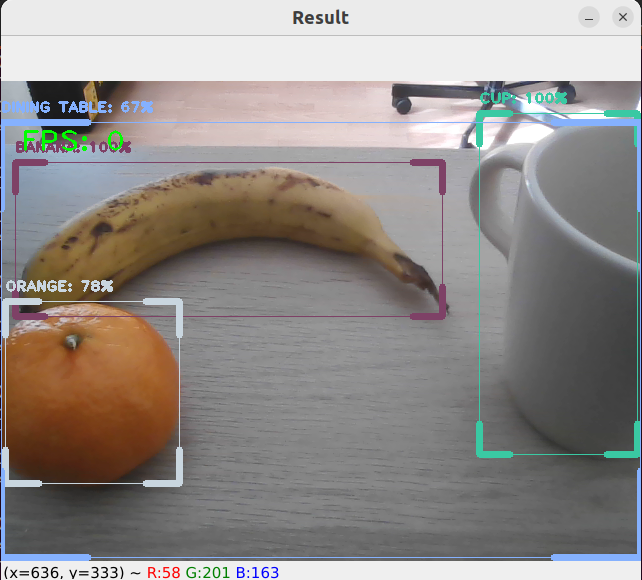
\includegraphics[height=50mm, width=70mm]{figs/webcam faster_rcnn_resnet50_v1_640x640_coco17_tpu-8.png}}
    	\end{center}
    	\caption{Modelo faster\_rcnn\_resnet50\_v1\_640x640\_coco17\_tpu-8 }
    	\label{fig:modelo_faster_rcnn_resnet50}
  	\end{figure}	
  	
\pagebreak

Después de haber llevado a cabo estas pruebas con los modelos de detección de objetos ssd\_mobilenet\_v2\_320x320\_coco17\_tpu-8, efficientdet\_d4\_coco17\_tpu-32 y faster\_rcnn\_resnet50\_v1\_640x640\_coco17\_tpu-8, y tras valorar que, el principal uso del modelo en la aplicación final sería la de llevar a cabo detecciones a tiempo real con una cámara, se escogió el modelo ssd\_mobilenet\_v2 para proseguir con los experimentos, incluso por delante de cualquiera de los otros dos modelos, ya que, a pesar de tener menor precisión y calidad de detección, destacaba principalmente por su elevada velocidad de procesamiento y su bajo consumo de recursos, gracias a su arquitectura ligera basada en MobileNetV2 y su tamaño de entrada reducido, haciéndolo especialmente adecuado para aplicaciones en tiempo real sobre hardware con capacidades limitadas, como puede ser un sistema de visión embarcado en un brazo robótico.\\

Para ello, y dado que para poder llevar a cabo la detección de fresas era necesario utilizar un modelo entrenado desde cero, para lo que se utilizó de guía el repositorio \textit{real\_time\_object\_detection\_cpu}\footnote{\url{https://github.com/haroonshakeel/real_time_object_detection_cpu/blob/main}}, creando y activando un nuevo entorno de Anaconda, donde se instalaron los paquetes y librerías necesarios para ello junto al Object Detection API de TensorFlow junto con Jupyter Notebook\footnote{\url{https://jupyter.org}}, un entorno computacional interactivo basado en web para crear cuadernos que contienen código en vivo, ecuaciones, visualizaciones y texto narrativo. \\

Completada la configuración del entorno, la instalación de todos los componentes, y el entrenamiento del modelo, se realizó una primera prueba de detección utilizando el modelo entrenado para comprobar si funcionaba, obteniendo las primeras predicciones en tiempo real sobre vídeo con fresas reales, y de este modo, poder llevar a cabo la batería de pruebas en las cuales se variaba tanto el número de fresas como las condiciones de luz, siendo los resultados de estos escenarios los que se muestran a continuación en la Figura \ref{fig:deteccion_Fresas_webcam_TF_ssdmobilenet}:
\pagebreak


\begin{figure}[H]
    \centering
    \subcapcentertrue
    % Fila 1
    \subfigure[Una única fresa con luz natural de día]{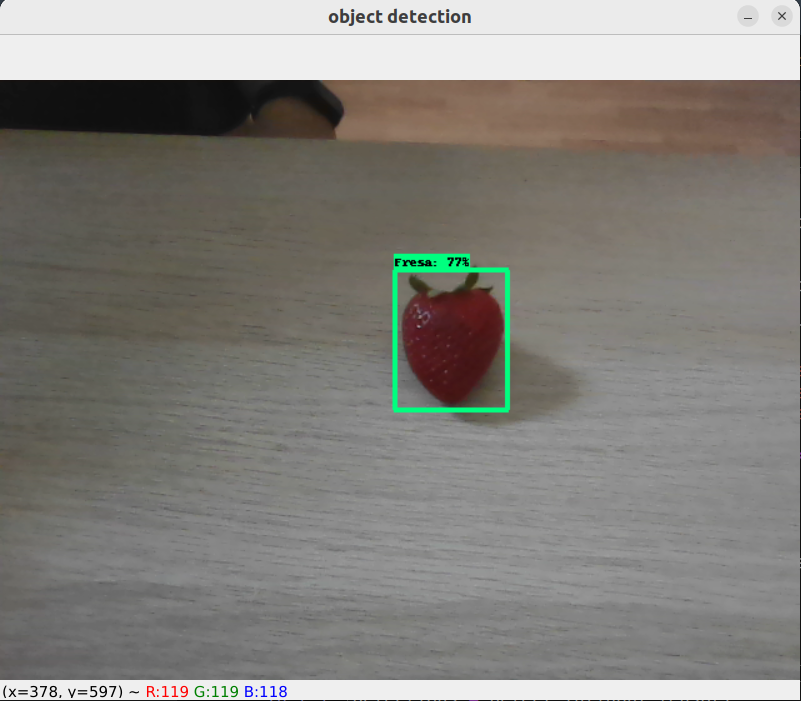
\includegraphics[width=0.30\textwidth]{figs/Deteccion una fresa luz natural dia JN.png}}
    \hspace{1mm}
    \subfigure[Una única fresa con luz artificial de día]{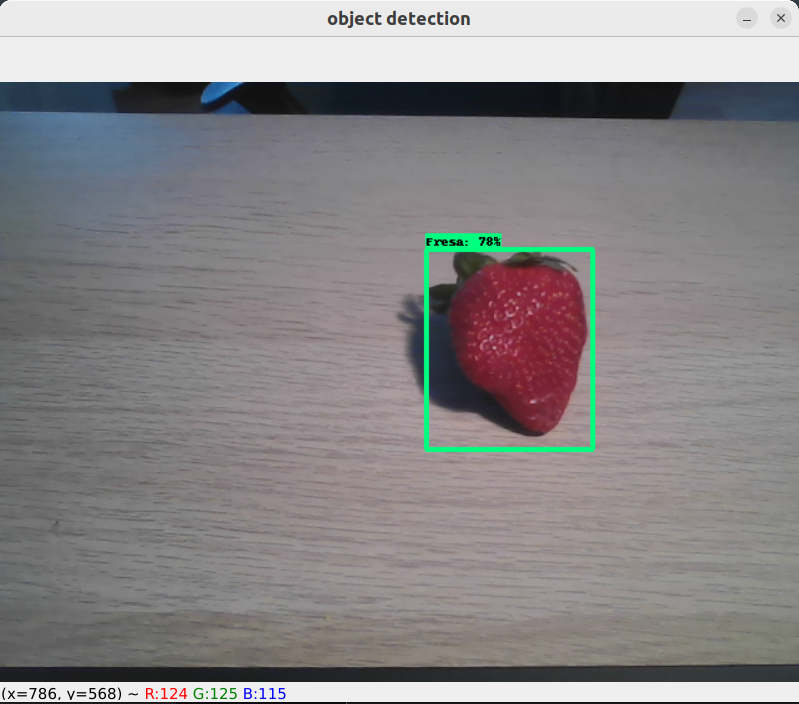
\includegraphics[width=0.30\textwidth]{figs/Deteccion una fresa luz artificial dia JN.png}}
    \hspace{1mm}
    \subfigure[Una única fresa con luz artificial de noche]{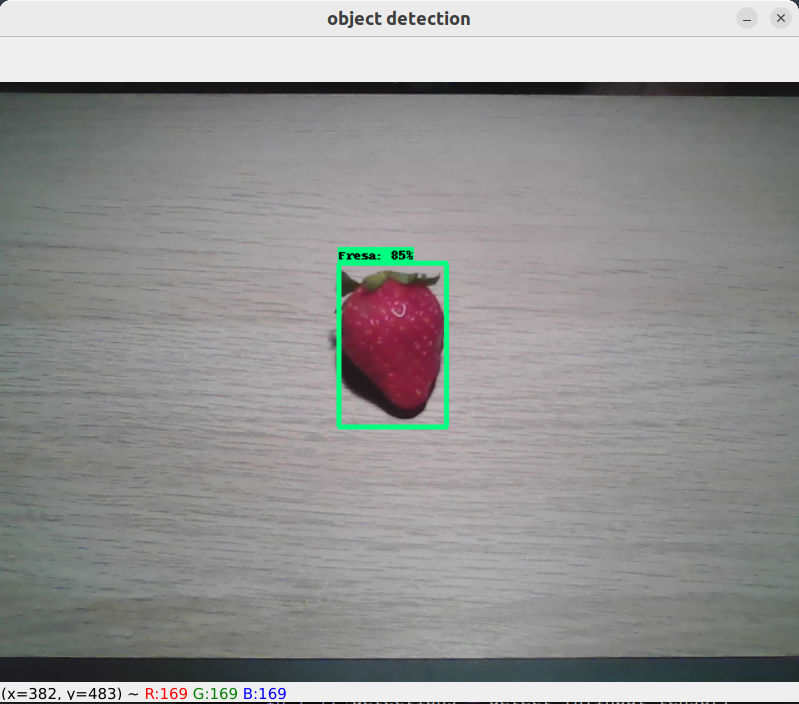
\includegraphics[width=0.30\textwidth]{figs/Deteccion una fresa luz artificial de noche JN.png}}

    \vspace{1mm} % Espacio vertical entre filas

    % Fila 2
    \subfigure[Varias fresas con luz natural de día]{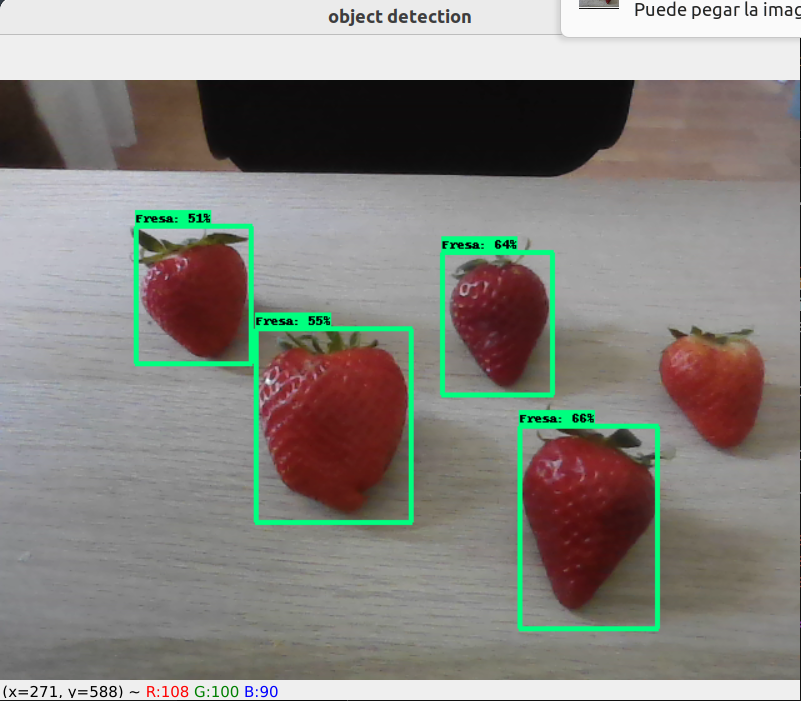
\includegraphics[width=0.30\textwidth]{figs/Deteccion varias fresas luz natural dia JN.png}}
    \hspace{1mm}
    \subfigure[Varias fresas con luz artificial de día]{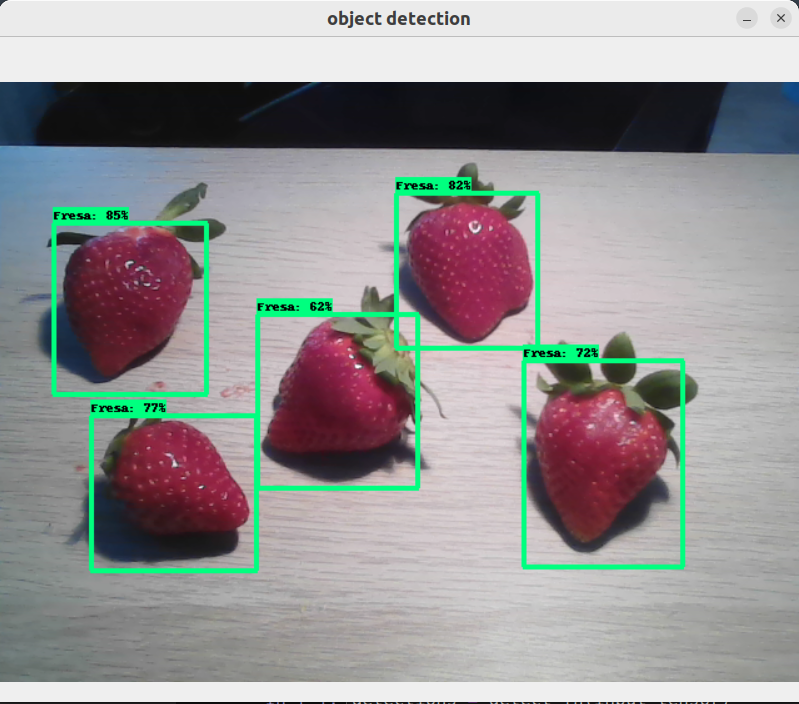
\includegraphics[width=0.30\textwidth]{figs/Deteccion varias fresas luz artificial dia JN.png}}
    \hspace{1mm}
    \subfigure[Varias fresas con luz artificial de noche]{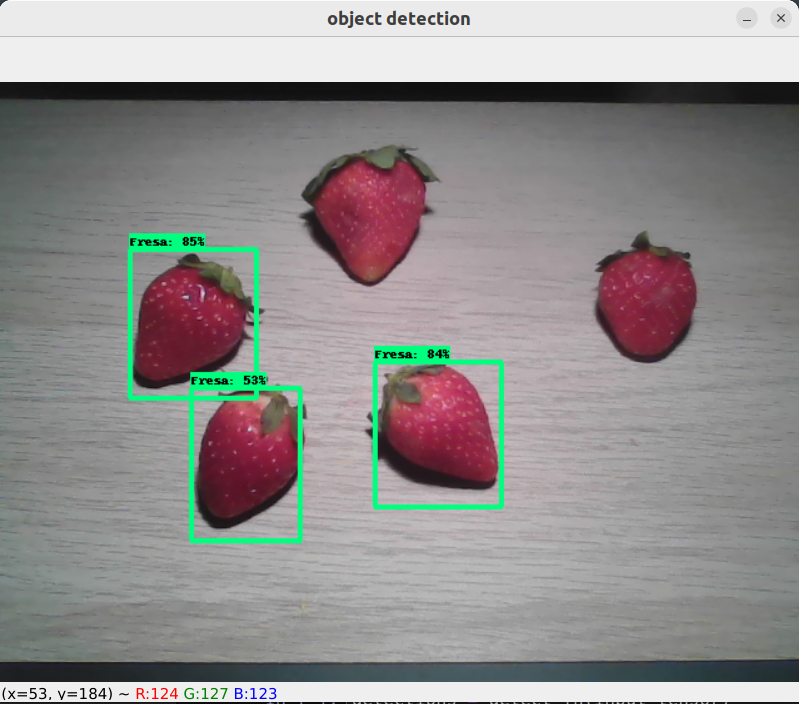
\includegraphics[width=0.30\textwidth]{figs/Deteccion varias fresas luz artificial de noche JN.png}}
    
    \caption{Detección de fresas en webcam con TensorFlow con modelos no pre-entrenados (ssd mobilenet v2 320x320)}
    \label{fig:deteccion_Fresas_webcam_TF_ssdmobilenet}
\end{figure}

Después de verificar la viabilidad y funcionamiento de estas pruebas, y de detectar en los resultados de estas pruebas que, con luz artificial existía un mayor porcentaje de confianza en las detecciones que con luz natural, se modificó el programa de detección para obtener más datos sobre estas detecciones y para poder mejorar el programa, incluyendo la instrucción mediante la cual se dejase de captar lo que se podía ver por la cámara del ordenador y se cerrase la ventana emergente correspondiente, a la que también se le cambió el nombre por \textit{strawberry detection}, calculando las coordenadas del punto central del recuadro de la detección, o añadiendo del cálculo de los FPS (fotogramas por segundo) en la ventana de detección en tiempo real (ver Figura \ref{fig:Coord_JN}), es decir, la medida de la frecuencia de cuadros en el vídeo, ya que representa la cantidad de imágenes individuales que se muestran en un segundo, midiendo la velocidad de procesamiento de los cuadros, siendo útil para comparar entre las distintas condiciones de detección, ya que un FPS más alto indica que se están procesando más cuadros por segundo, lo que generalmente se considera deseable para aplicaciones en tiempo real.\\ 

  \begin{figure}[H]
     \centering
     \begin{center}
       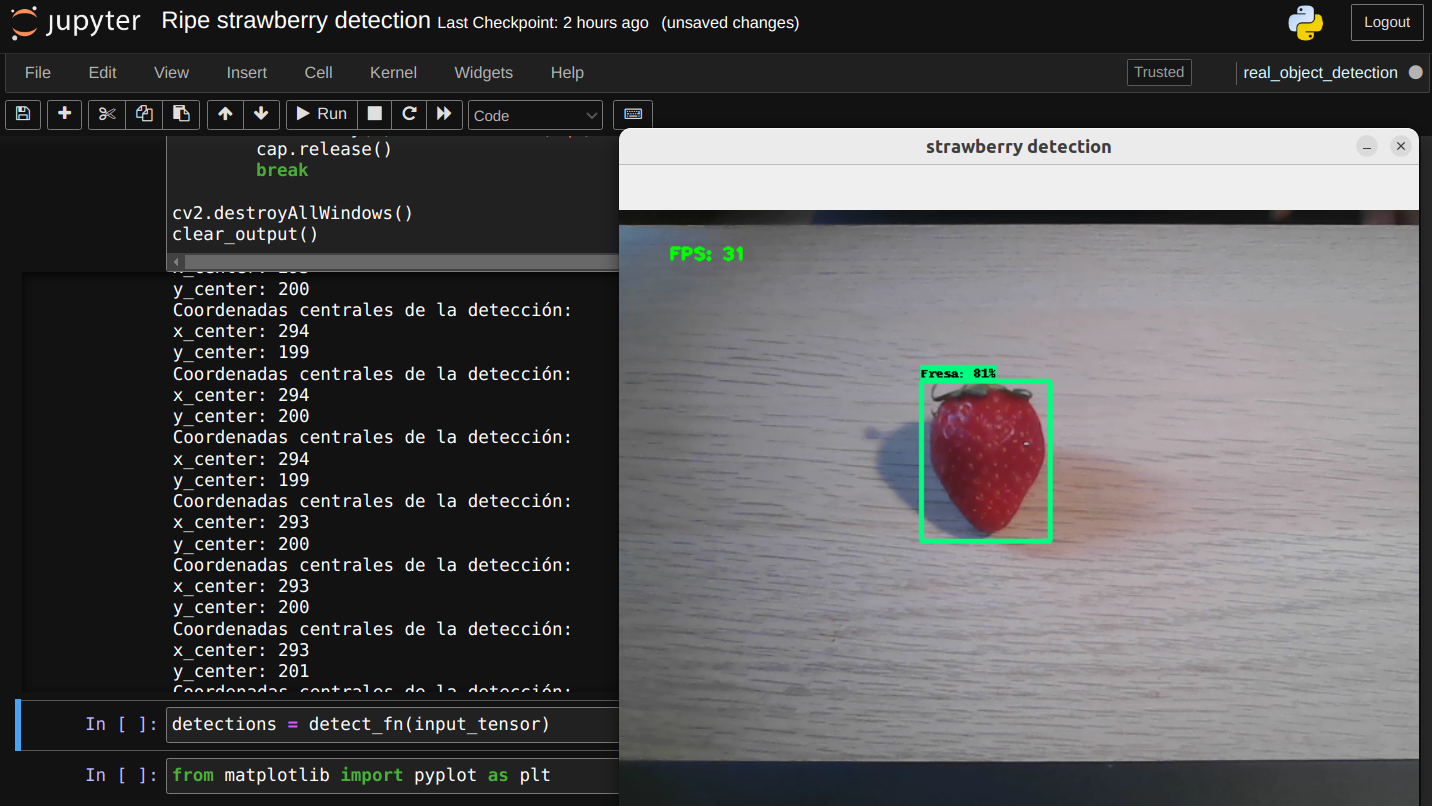
\includegraphics[width=11cm]{figs/Coordenadas centrales deteccion JN.png}
     \end{center}
     \caption{Deteccion de fresas en Jupyter Notebook}
    \label{fig:Coord_JN}
  \end{figure}

Aunque Jupyter Notebook ofrecía un entorno interactivo y muy útil no era recomendable utilizarlo como entorno de ejecución para aplicaciones estables conectadas a robots, puesto que su diseño está orientado principalmente a tareas de análisis, visualización y prototipado, donde el usuario interactúa continuamente con el entorno mediante la ejecución manual de celdas, suponiendo una limitación importante para sistemas robóticos, los cuales requieren un comportamiento determinista, autónomo y ejecutable sin supervisión constante. Una de las principales desventajas de Jupyter en este contexto es su modelo de ejecución no lineal, ya que, a diferencia de un script en Python, donde el flujo de ejecución es siempre secuencial y controlado, en un notebook es posible ejecutar fragmentos de código en cualquier orden, pudiendo provocar desincronización en las variables del programa y errores difíciles de detectar, especialmente críticos en aplicaciones donde se controla hardware, se toman decisiones en tiempo real o se actúa sobre el entorno físico. Además, a pesar de que Jupyter Notebook utiliza el lenguaje Python y puede ejecutar cualquier código compatible, su arquitectura está basada en un servidor web local que muestra la interfaz en un navegador, lo que implica que, aunque no necesita conexión a Internet, sí requiere iniciar un servidor HTTP en el sistema local, por lo que sería necesario implementar manualmente un servidor adicional dentro del propio notebook. Esto introduce una complejidad innecesaria y un entorno frágil, ya que tanto el servidor adicional como el entorno Jupyter deben mantenerse activos, y cualquier error o bloqueo en una celda puede interrumpir toda la operación.\\

Por todas estas razones, aunque Jupyter Notebook puede ser muy útil durante las fases iniciales del desarrollo para validar algoritmos de visión o procesado de datos, la implementación definitiva de un sistema conectado a un robot debe realizarse mediante scripts de Python, permitiendo un mayor control sobre el flujo de ejecución, una integración más sencilla en sistemas de control y producción, y una mayor robustez operativa, aspectos esenciales en el desarrollo de aplicaciones robóticas fiables.




\section{Detección con YOLOv3 y PyTorch}
\label{exp_seleccion_algoritmo}

Para poder comprobar las diferencias en un ejemplo práctico a la hora de detectar objetos entre PyTorch y TensorFlow, y de esta manera poder escoger una de las dos bibliotecas para el desarrollo del modelo de aprendizaje automático y aprendizaje profundo en este proyecto, se decidió crear de nuevo un entorno de Anaconda y probar a detectar objetos en imágenes utilizando Tensorflow.

\subsection{Pruebas con modelos preentrenados}
\label{sec:Pruebas_modelo_preentrenado_Pytorch}

Después de realizar la lectura \textit{You Only Look Once: Unified, Real-Time Object Detection}\cite{Redmon16}, se replicó lo que se exponía en dicho artículo con la cámara integrada del ordenador portátil, mediante un programa en Python y usando la librería Open Source Computer Vision Library (OpenCV) mediante la biblioteca Pytorch. Este programa, partiendo del \textit{feed} de la propia webcam, descomponía el vídeo en imágenes o cuadros, alimentando a la red neuronal (en este caso YOLOv3), que recibía esta detección y se procesaba con OpenCV, dibujando los recuadros o \textit{bounding box} alrededor de los objetos que se detectaban en vivo.\\

Para ello, primero se realizó la instalación de Anaconda para poder crear un ambiente de trabajo independiente y así evitar problemas entre las versiones de los paquetes necesarios para la ejecución de estas pruebas, y posteriormente se instaló OpenCV. Se clonó el repositorio \textit{deteccion-objetos-video}\footnote{\url{https://github.com/puigalex/deteccion-objetos-video}} basado en el proyecto \textit{PyTorch-YOLOv3}\footnote{\url{https://github.com/eriklindernoren/PyTorch-YOLOv3}} para correr detección de objetos sobre video y se siguieron los pasos detallados en el archivo README.
Una vez instalado todo, se probó a utilizar varios objetos y posteriormente varias frutas simultáneamente para verificar que el modelo las diferenciaba correctamente y las detectaba, tal y como se muestra en la Figura \ref{fig:Deteccion_Pytorch}.

  \begin{figure}[H]
    \begin{center}
      \subcapcentertrue
      \subfigure[Prueba deteccion de objetos con Pytorch]{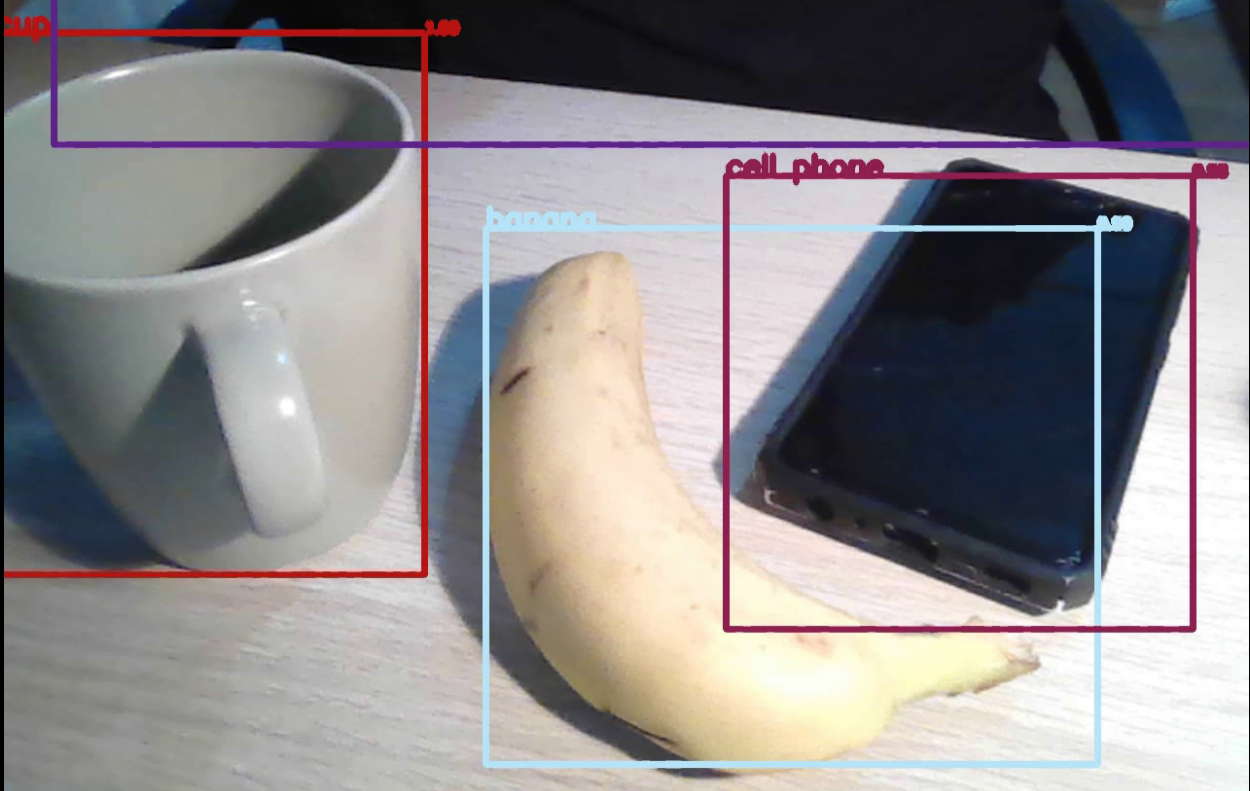
\includegraphics[width=73mm]{figs/Prueba deteccion de objetos con pytorch.png}}
      \hspace{2mm}
      \subfigure[Prueba deteccion de frutas con Pytorch]{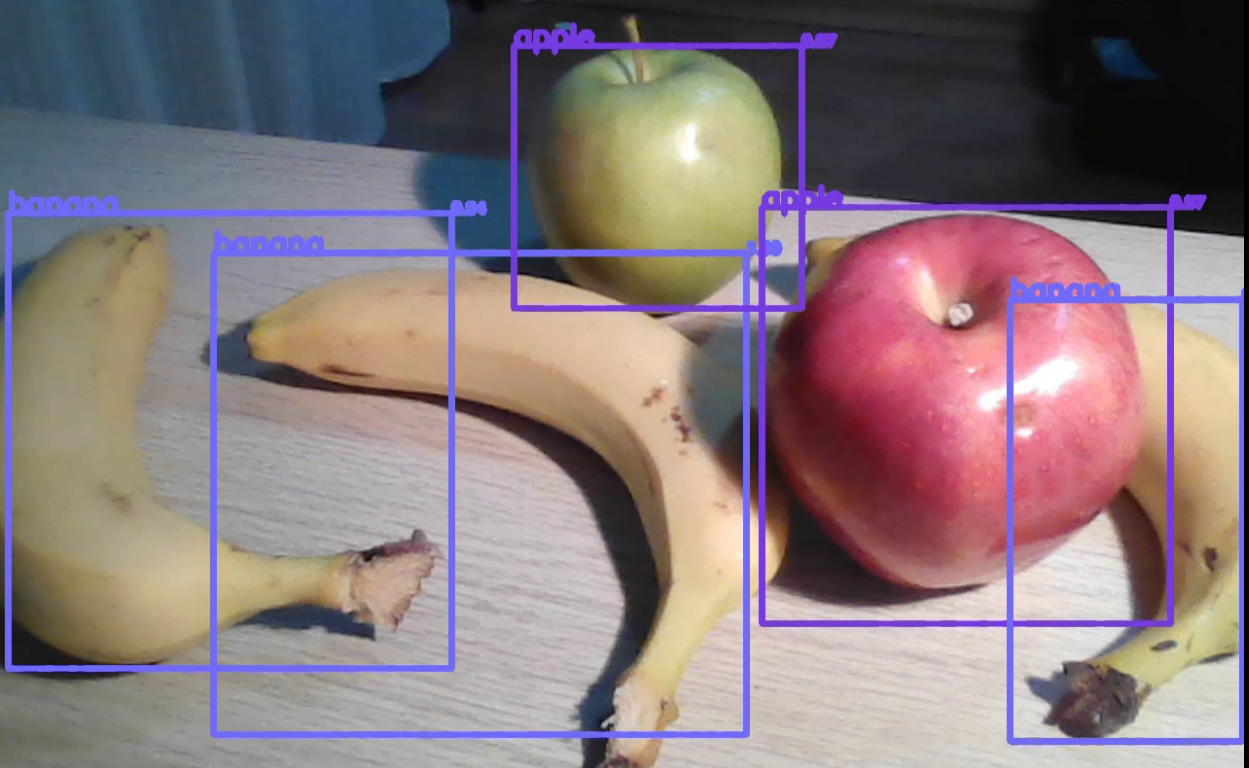
\includegraphics[width=75mm]{figs/Prueba derteccion de frutas con pytorch.png}}
    \end{center}
    \caption{Deteccion con Pytorch}
    \label{fig:Deteccion_Pytorch}
  \end{figure}
  
\subsection{Entrenamiento del modelo}
\label{sec:entrenamiento_modelo_Pytorch_Python}


Debido a que, tras la detección de las posiciones de las fresas mediante el programa de Jupyter Notebook, no se puede trabajar directamente con ellas y enviarlas al robot, ya que Jupyter Notebook está basado en web, por lo que haría falta un servidor web intermediario para esto, tal y como se explicó en el apartado anterior, se intentó llevar a cabo la elaboración del programa de detección en Python, para que de este modo se pudieran enviar al brazo robótico directamente las coordenadas, al estar trabajando en local y tener todo el código unificado. Además, se sustituyó TensorFlow por PyTorch como biblioteca de desarrollo del modelo de visión, basándose en que PyTorch ofrece una sintaxis más intuitiva y cercana a la programación en Python puro, lo que facilita su integración con scripts que deben ejecutarse en tiempo real junto con otros módulos, como los encargados de la comunicación con el robot, además de que PyTorch presenta una curva de aprendizaje más suave para depuración y prototipado rápido, y proporciona una mayor facilidad a la hora de exportar modelos, optimizarlos o ajustarlos dinámicamente durante la ejecución, resultando ser más adecuado para un sistema unificado, local y modular que debe ejecutarse de forma autónoma, sin depender de interfaces gráficas ni entornos web como Jupyter.\\

Para ello se tomó como referencia y ayuda los repositorios \textit{Real Time Emotion Detection for Low Cost Robot in ROS}\footnote{\url{https://github.com/jamarma/emotion_detection_ros}} y \textit{Detección de objetos en vídeo}\footnote{\url{https://github.com/puigalex/deteccion-objetos-video}} y se creó un entorno nuevo en Anaconda llamado \textit{deteccionobj}.\\

Durante el entrenamiento del modelo, surgieron varios códigos de error relacionados con el etiquetado de las imágenes utilizadas para esto, por lo que se decidió etiquetarlas de nuevo mediante el programa labelImg (Figura \ref{fig:labelImg_Fresas}), tal y como se había hecho anteriormente con TensorFlow.

 \begin{figure}[H]
     \centering
     \begin{center}
       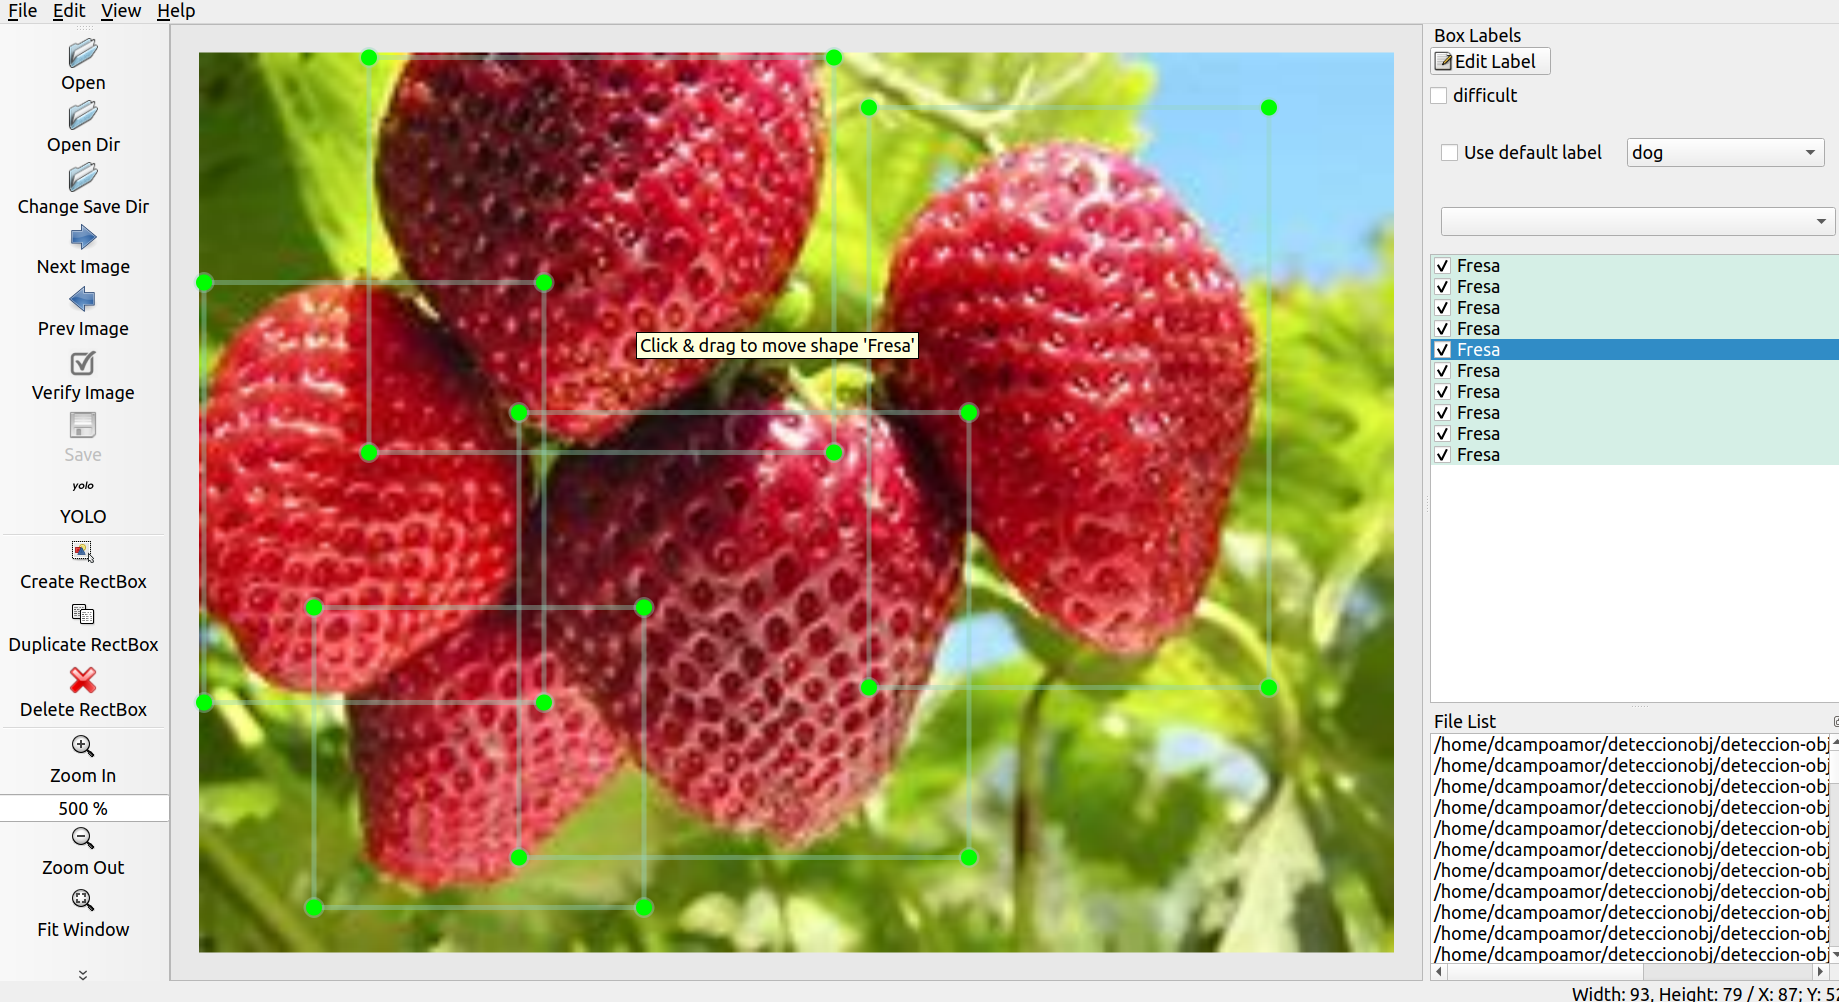
\includegraphics[width=11cm]{figs/labelImg Fresa.png}
     \end{center}
     \caption{Etiquetado de las imágenes con labelImg}
    \label{fig:labelImg_Fresas}
  \end{figure}

Finalizado el proceso de etiquetado de 432 imágenes, se almacenaron en la carpeta \textit{labels} los archivos que incluían tanto el número de clase, identificado con el valor 0, correspondiente a la única clase considerada, "Fresa",  como las coordenadas que delimitaban la ubicación del objeto dentro de cada imagen. Con esta información organizada, se procedió al entrenamiento del modelo utilizando la arquitectura Darknet-53, implementada en el framework Darknet, más concretamente se empleó el archivo darknet53.conv.74, correspondiente a las primeras 74 capas de la red preentrenadas con pesos convolucionales, lo cual permitió una inicialización eficiente y evitó entrenar el modelo YOLO desde cero.\\

Para el entrenamiento, se configuró el parámetro batch\_size con un valor de 2, debido a las limitaciones de capacidad de la tarjeta gráfica empleada, lo que implicó que las imágenes se procesaran de dos en dos por iteración. Además, al finalizar cada época del entrenamiento, entendida como el momento en que la red ha procesado y actualizado todos los ejemplos del conjunto de entrenamiento, se generó un checkpoint con los pesos actuales del modelo, almacenado en la carpeta correspondiente, dando lugar a un total de 100 checkpoints al concluir el proceso dado que el entrenamiento fue configurado por defecto para ejecutarse durante 100 épocas.

\subsection{Calibrado de la cámara}
\label{sec:Calibrado_camara}

Con el fin de optimizar la detección de objetos mediante YOLOv3 y PyTorch, se procedió a la calibración de la cámara web de Logitech C270, determinando sus parámetros intrínsecos y la transformación de su sistema de coordenadas respecto al entorno. Para ello, se utilizaron 20 imágenes de un patrón de tablero de ajedrez en diferentes posiciones, tomadas con la cámara a calibrar, mediante las cuales, y a través del uso del programa \textit{PiCamCalibrator.py}, se obtenían estos valores de la matriz K, como muestra la Figura \ref{fig:calibracion_camara}. 

 \begin{figure}[H]
    \begin{center}
      \subcapcentertrue
      \subfigure[Chess board]{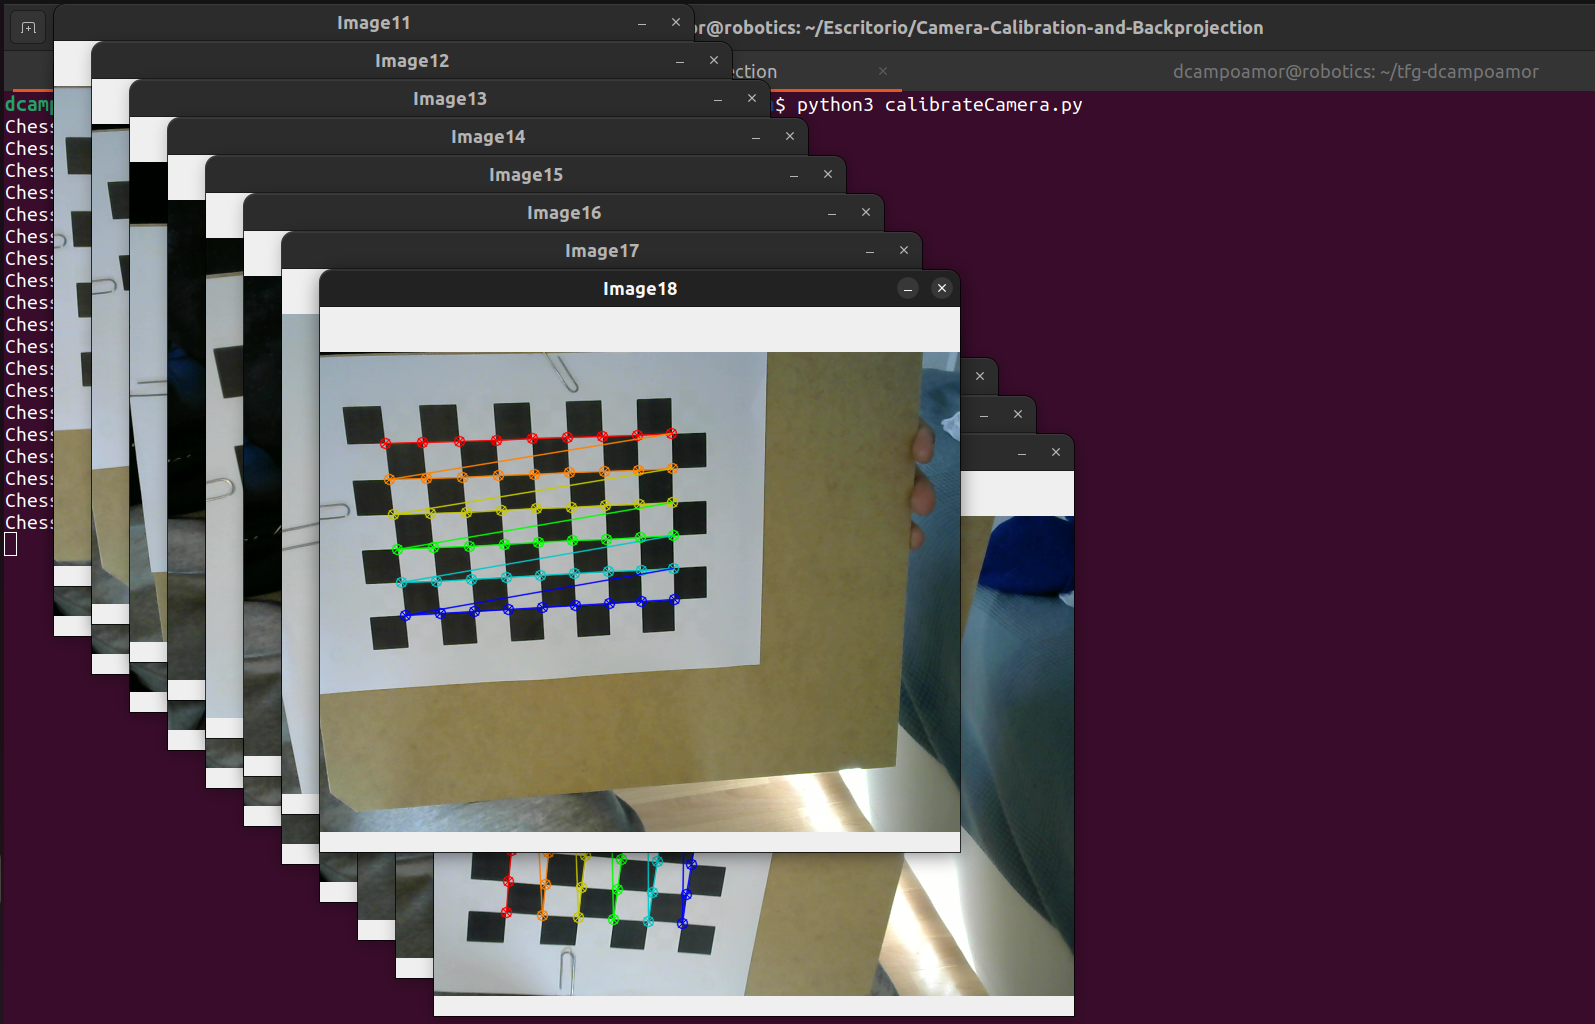
\includegraphics[height=40mm, width=73mm]{figs/calibrateCamera.png}}
      \hspace{2mm}
      \subfigure[Parámetros intrínsecos de la cámara]{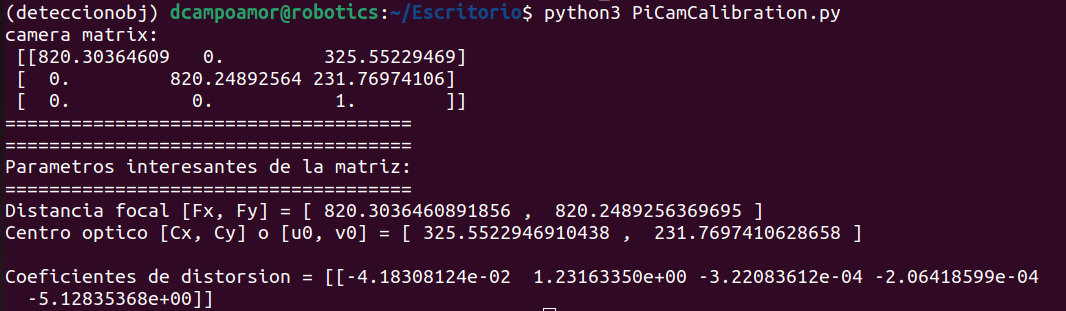
\includegraphics[height=40mm, width=75mm]{figs/matriz K camara.png}}
    \end{center}
    \caption{Calibración de la cámara C270 de Logitech}
    \label{fig:calibracion_camara}
  \end{figure}

Para corroborar si esta primera calibración de la cámara C270 de Logitech había sido buena, se llevaron a cabo diez calibraciones más para comprobar los resultados entre sí con diferentes imágenes tomadas con el mismo \textit{chess board}, siendo los valores tomados para la programación, la media aritmética entre todas las mediciones.

Junto con las matrices de Rotación R y la matriz de Traslación T de la cámara, se realizó el cálculo de la transformación del sistema de coordenadas que viene definido por la multiplicación de las tres matrices, para lo cuál, se instaló la cámara en un trípode, cuya altura al plano mesa conocíamos, y con una inclinación de la cámara medida mediante la aplicación de ERGONAUTAS RULER - Medición de ángulos en fotografías y vídeos\footnote{\url{https://www.ergonautas.upv.es/herramientas/ruler/ruler.php}} de la Universidad Politécnica de Valencia.

\subsection{Pruebas detección de fresas en tiempo real}
\label{sec:Pruebas_Fresas_Pytorch}

Una vez con el modelo entrenado, se realizaron las primeras pruebas utilizando Python de detección de fresas en tiempo real, para las que se utilizó la cámara integrada del ordenador portátil e imágenes de fresas en el móvil, tal y como se muestra en la Figura \ref{fig:primerasdetecciones_Python}, y a partir de las cuales se modificaron tanto el grosor del nombre de la clase a detectar como el threshold de la detección mostrado en la ventana emergenteen con OpenCV, ajustándolde tal manera quemo argumento que pudieran ser más legibles en el programa.

 \begin{figure}[H]
     \centering
     \begin{center}
       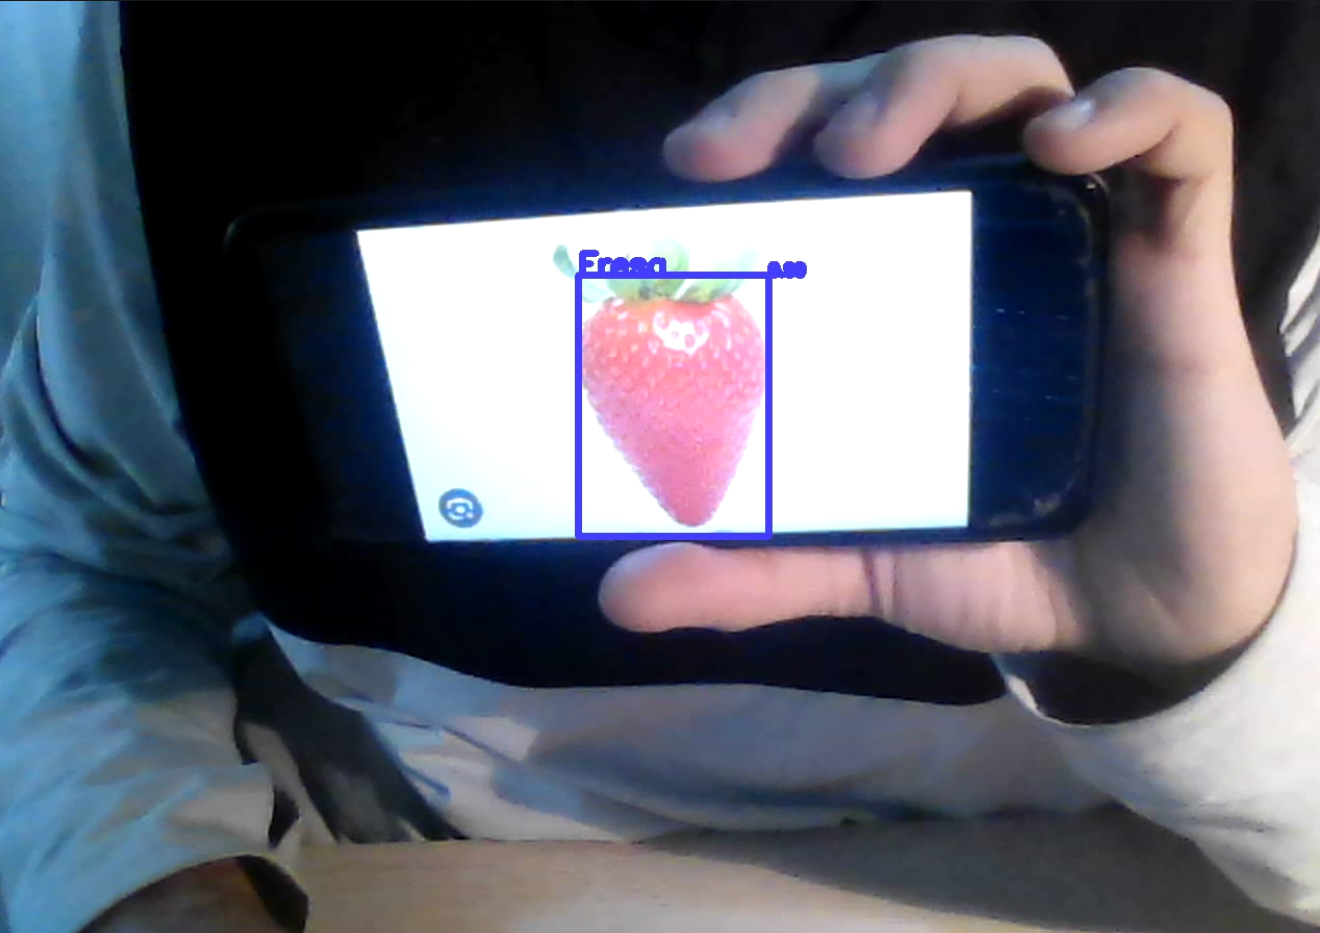
\includegraphics[width=80mm]{figs/deteccion_video fresa en foto.png}
     \end{center}
     \caption{Primeras pruebas de detección con PyTorch y Python}
    \label{fig:primerasdetecciones_Python}
  \end{figure}

Sobre esta primera versión se fue modificando el código para poder añadir más funcionalidades al sistema, como la incorporación de un fragmento diseñado para almacenar dinámicamente las coordenadas centrales de los recuadros de las fresas detectadas por el modelo en una lista, y, dado que la versión inicial del script no consideraba la posible redundancia en la detección, es decir, la identificación múltiple de un mismo objeto debido a ligeras variaciones en la posición, también se incorporó un criterio de tolerancia espacial, que permitiera verificar si una nueva detección se encontraba a una distancia euclidiana inferior al umbral respecto a alguna de las posiciones ya registradas, y en tal caso, la nueva posición no se añadiría a la lista, evitando así duplicidades en las detecciones.


\section{Pruebas con el robot real}
\label{Pruebas_UR}

Una vez decidido que la mejor opción para la detección de fresas era utilizar el modelo YOLOv3, implementado con TensorFlow en Python, se procedió a realizar las primeras pruebas con el brazo robótico de Universal Robots. El objetivo principal de estas pruebas fue comprobar la correcta comunicación entre el sistema de detección y el robot, así como validar la precisión del movimiento del robot hacia las posiciones detectadas en el plano, permitieron identificar posibles ajustes en la calibración y evaluar el funcionamiento del sistema en un entorno controlado antes de su aplicación conjunta.

En primer lugar, se programó en la Interfaz Gráfica de Usuario (IGR) del robot un ejemplo para ir a una posición fija que simulaba una posición en el espacio determinada por un sistema de visión externo, siendo esto la base del programa final del propio robot, ya que, tras esto, se añadieron al programa las líneas necesarias para poder abrir la comunicación con un servidor, leer los datos de este.



